\documentclass[acmtocl,acmnow]{acmtrans2m}

\usepackage{graphicx}

\newtheorem{theorem}{Theorem}[section]
\newtheorem{conjecture}[theorem]{Conjecture}
\newtheorem{corollary}[theorem]{Corollary}
\newtheorem{proposition}[theorem]{Proposition}
\newtheorem{lemma}[theorem]{Lemma}
\newdef{definition}[theorem]{Definition}
\newdef{remark}[theorem]{Remark}


           
\markboth{Nigel Stanger}{...}

\title{Scalability of Methods for Online Geovisualisation of Web Site Hits}
            
\author{NIGEL STANGER \\ University of Otago}
            
\begin{abstract} 
A common technique for visualising the geographical distribution of
web site hits is to geolocate the IP addresses of hits and plot them on
a world map. This is typically achieved by dynamic generation of images
on the server. In this paper we compare this method with two others:
overlaying CSS-enabled HTML on an underlying image and using Google
Maps. The results show that all three methods are suitable for small
data sets, but that the latter two methods do not scale well to large
data sets.
\end{abstract}
            
\category{C.4}{Performance of Systems}{Performance attributes}
\category{C.2.4}{Computer-Communication Networks}{Distributed Systems}[distributed applications]
\category{H.3.5}{Information Storage and Retrieval}{Online Information Services}[web-based services]
            
\terms{Experimentation, Measurement, Performance} 
            
\keywords{geolocation, geovisualisation, scalability, GD, Google Maps}
            
\begin{document}


\bibliographystyle{acmtrans}

            
\begin{bottomstuff} 
Author's address: N. Stanger, Department of Information Science,
University of Otago, PO Box 56, Dunedin 9054, New Zealand.
\end{bottomstuff}
            
\maketitle


\section{Introduction}
\label{sec-introduction}

When running a web site, it is quite reasonable to want information on
the nature of traffic to the site. For example, an e-commerce site might
wish to determine the geographical distribution of visitors to its site,
so that it can decide where best to target its marketing resources. One
approach to doing so is to plot the geographical location of web site
hits on a map. Geographical information systems (GIS) were already being
used for these kinds of purposes prior to the advent of the World Wide
Web \cite{Beau-JR-1991-GIS}, and it is a natural extension to apply
these ideas to online visualisation of web site hits.

Our interest in this area derives from implementing a pilot digital
institutional repository at the University of
Otago\footnote{\url{http://eprints.otago.ac.nz/}} in November 2005
\cite{Stan-N-2006-running}, using the GNU EPrints repository management
software\footnote{\url{http://www.eprints.org/}}. The repository quickly
attracted interest from around the world and the number of abstract
views and document downloads began to steadily increase. We were
obviously very interested in monitoring this increase, particularly with
respect to where in the world the hits were coming from. The EPrints
statistics software developed at the University of Tasmania
\cite{Sale-A-2006-stats} proved very useful in this regard, providing us
with detailed per-eprint and per-country download statistics; an example
of the latter is shown in Figure~\ref{fig-tas-stats}. However, while
this display provides a numerical ranking of the number of hits from
each country, it does not provide any visual clues as the distribution
of hit sources around the globe.


\begin{figure}
	\begin{center}
		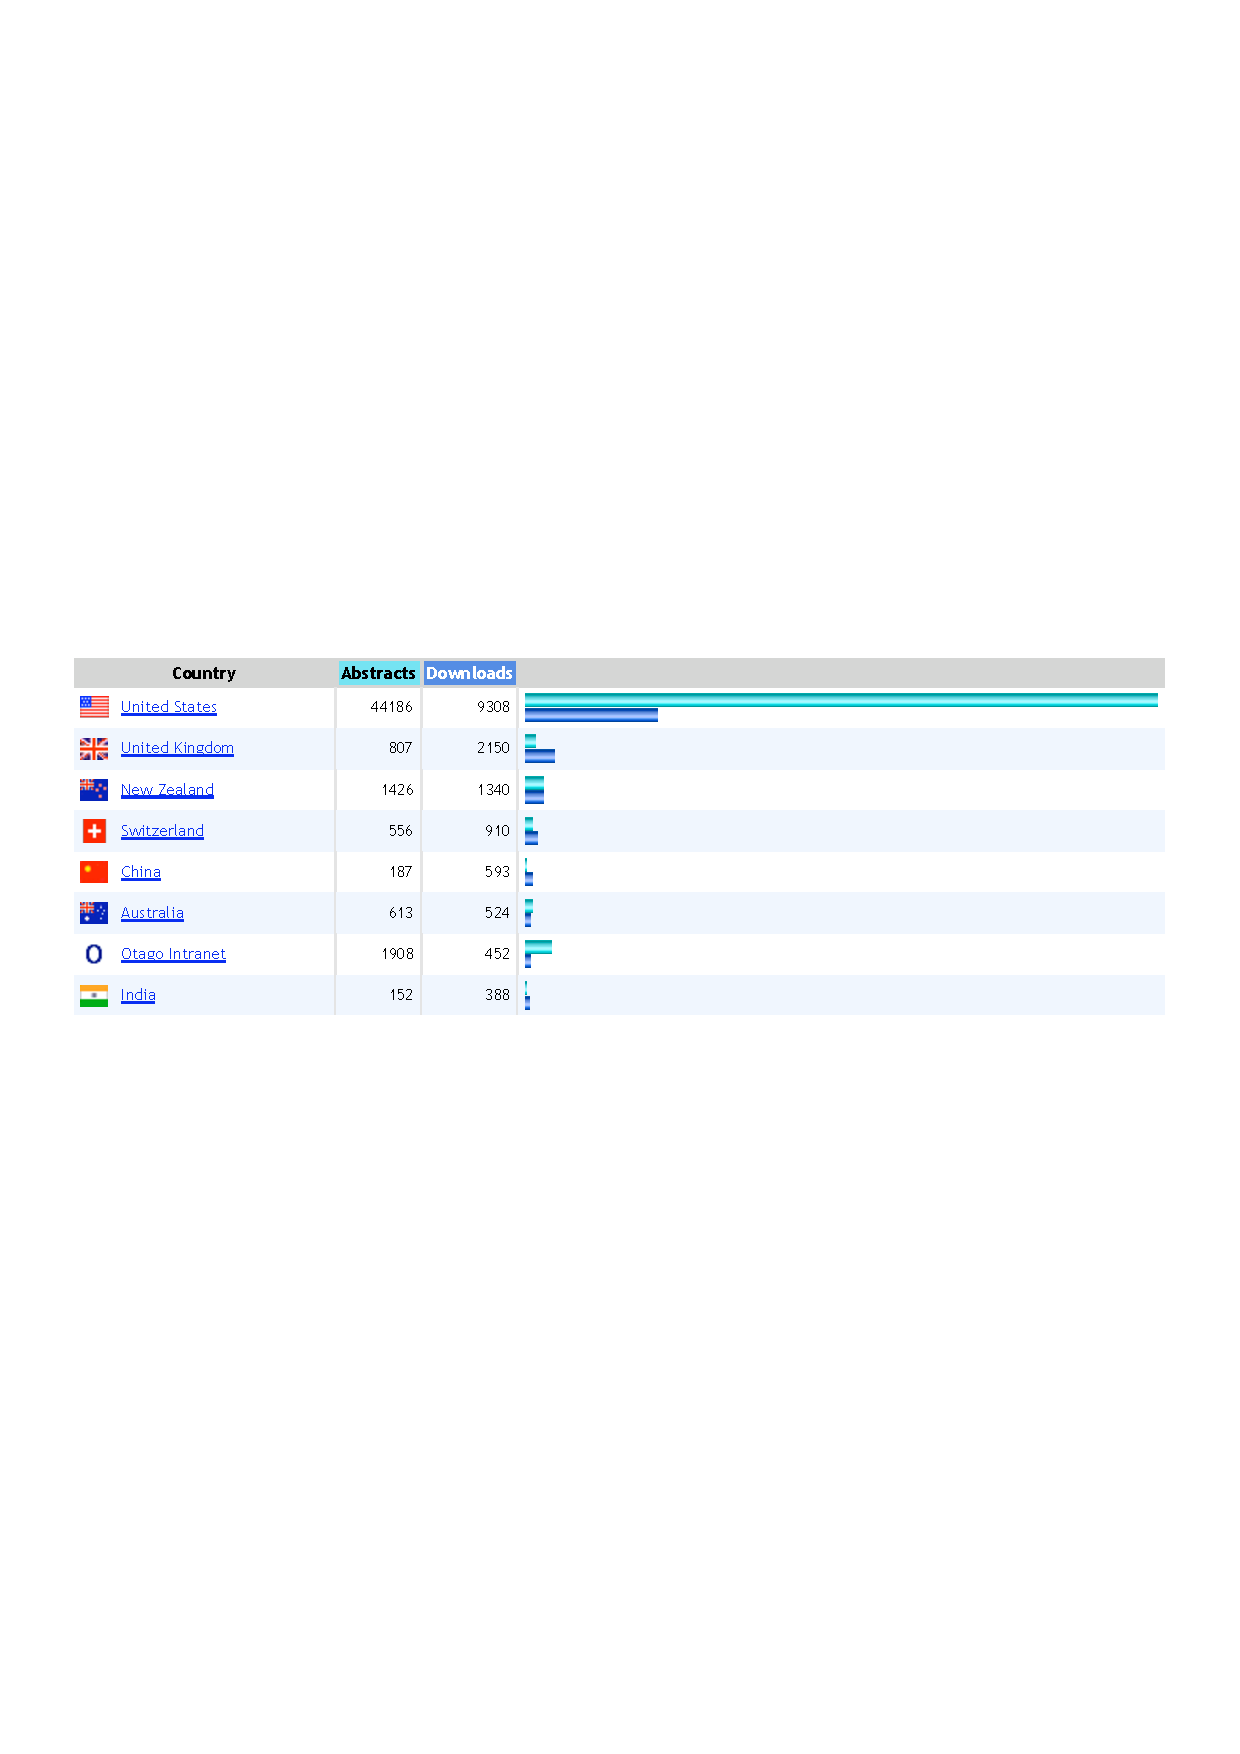
\includegraphics[scale=0.65]{tasmania_stats}
	\end{center}
	\caption{A portion of the by-country display for the Otago EPrints
	repository, generated by the Tasmania statistics software.}
	\label{fig-tas-stats}
\end{figure}


We therefore began to explore various techniques for plotting our
repository hit data onto a world map, with the aim of adding this
capability to the Tasmania statistics package. Our preference was for a
technique that could be used within a modern web browser without the
need to manually install additional client software, thus providing us
with the widest possible audience and reducing the impact of wide
variation in client hardware and software environments \cite[pp.\
27--28]{Offu-J-2002-quality}.

There have been several prior efforts to plot web activity
geographically. \citeN{Lamm-SE-1996-webvis} developed a sophisticated
system for real-time visualisation of web traffic on a 3D globe, but
this was intended for use with a virtual reality interface, thus
limiting its general applicability. \citeN{Papa-N-1998-Palantir}
describe a similar system (Palantir) that is written in Java, and thus
able to be run within a web browser, asssuming that a Java virtual
machine is available. \citeN[pp.\ 100--103]{Dodg-M-2001-cybermap}
describe these and several other related systems.

These early systems suffered from a distinct limitation in that there
was no public infrastructure in place for geolocating IP addresses (that
is, translating them into latitude/longitude coordinates). They
generally used \texttt{whois} lookups or parsed the domain name in an
attempt to guess the country of origin, but these produced fairly crude
results. Locations outside the United States were typically aggregated
by country and mapped to the capital city
\cite{Lamm-SE-1996-webvis,Papa-N-1998-Palantir,Jian-B-2000-cybermap}.
Reasonably accurate databases were commercially available at the time
\cite[p.\ 1466]{Lamm-SE-1996-webvis}, but were not available to the
public at large, thus limiting their utility.

The situation has improved considerably in the last five years, however,
with the advent of freely available and reasonably accurate geolocation
databases\footnote{Such as \url{http://www.maxmind.com/} or
\url{http://www.ip2location.com/}.} with worldwide coverage and
city-level resolution. For example, Maxmind's \emph{GeoLite City}
database is freely available and claims to provide ``60\% accuracy on a
city level for the US within a 25 mile radius''
\cite{Maxm-G-2006-GeoLiteCity}. Their commercial \emph{GeoIP City}
database claims 80\% accuracy for the same parameters.

Based on the literature, it appeared that a Palantir-style model would
be suitable for our purposes. The Palantir software itself appears to no
longer be available, but we would probably not have used it anyway as it
requires the client machine to have a Java virtual machine installed.
Palantir worked by plotting web hits directly onto a base map image,
then displaying the composite image, all within a client-side Java
applet. However, the basic technique can just as easily be implemented
as a server-side application that returns a bitmap image to the client.
We shall henceforth refer to this technique as \emph{image generation};
it will be discussed further in Section~\ref{sec-imagegen}.

However, there are alternative techniques that have become possible only
relatively recently, and are therefore less likely to be in wide use.
One possible technique is to load a base image into the browser, then
overlay points onto the image using using absolutely positioned HTML
\verb|<DIV>| elements. This technique raises the potential for a more
GIS-like style of interaction with the map, with multiple layers that
can be activated and deactivated as necessary.  We refer to this
technique as \emph{HTML overlay}; it will be discussed further in
Section~\ref{sec-overlay}.

Another recent development is the release of the Google Maps API
\cite{Goog-M-2006-maps}, which enables web developers to easily embed
dynamic, interactive maps within web pages. These maps have an obvious
visual appeal and provide quite powerful interactive functionality
(including pan and zoom) out of the box. They also offer significant
customisability to the developer. This technique will be discussed
further in Section~\ref{sec-google}.

The identification of these three techniques immediately raised the
question of which was the best for our purposes. Of greatest concern was
whether these techniques could scale to a large number of points, as
scalability is a key issue for web applications in general \cite[p.\
28]{Offu-J-2002-quality}, and online activity visualization in
particular \cite[p.\ 50]{Eick-SG-2001-sitevis}. For example, at the time
of writing the Otago EPrints repository had been accessed from over
10,000 distinct IP addresses, each potentially representing a distinct
geographical location. Taking into consideration the type of hit
(abstract view versus document download) increased that figure to nearly
13,000. Ideally we wanted a technique that could plot a large number of
points as quickly as possible.

We therefore set about testing the scalability of the three techniques
to determine how well each technique handled large numbers of points. A
series of experiments was conducted using each technique with
progressively larger data sets, and the elapsed time and memory usage
were measured. The experimental design is discussed in
Section~\ref{sec-experiment}.

Our initial intuition was that the image generation technique would
prove the most scalable, and this was borne out by the results of the
experiments, which show that image generation scales reasonably well to
very large numbers of points. The other two techniques proved to be
reasonable for relatively small numbers of points (generally less than
about 500), but their performance deteriorated rapidly beyond this. The
results are discussed in more detail in Section~\ref{sec-results}.


\section{The techniques in more detail}
\label{sec-techniques}

In this section we discuss in more detail each of the three techniques
outlined in the previous section. For each technique, we examine how the
technique works in practice, its implementation requirements, its
relative advantages and disadvantages, and any other issues peculiar
to the technique.


\subsection{Image generation}
\label{sec-imagegen}

As noted earlier, this technique works by directly plotting geolocated
IP addresses onto a base map image, then displays the composite image at
the client, as shown in Figure~\ref{fig-image}. It requires two
additional pieces of software: one that can create and manipulate bitmap
images programmatically (for example, the GD image
library\footnote{\url{http://www.boutell.com/gd/}}); and one that can
transform raw latitude/longitude coordinates into projected map
coordinates on the base map (for example, the PROJ.4 cartographic
projections library\footnote{\url{http://www.remotesensing.org/proj/}}).


\begin{figure}
	\begin{center}
		\includegraphics[width=0.95\textwidth,keepaspectratio]{gd_map}
	\end{center}
	\caption{Sample output from the image generation technique.}
	\label{fig-image}
\end{figure}


The Palantir system implemented a distributed architecture for this
technique, where the source data were generated at the server and the
map was generated by a Java applet at the client
\cite{Papa-N-1998-Palantir}. Alternatively, the map image can be
generated entirely on the server. Both architectures are illustrated in
Figure~\ref{fig-image-architecture}. We have adopted the latter approach
in our experiments (server-side image generation), as the former would
require installing additional software at the client (for generating
images and performing cartographic projection operations).


\begin{figure}
	\caption{Distributed vs.\ server-side architectures for the image
	generation technique.}
	\label{fig-image-architecture}
\end{figure}


This technique provides some distinct advantages. If a server-side
architecture is adopted, the technique is relatively simple to implement
and is fast at producing the final image, mainly because it uses
existing, well-established technologies. It is also bandwidth efficient:
the size of the generated map image is determined by the total number of
pixels and the compression method used, rather than by the number of
points plotted. The amount of data generated should therefore remain
more or less constant, regardless of the number of points plotted.

This technique also has some disadvantages, however. First, a suitable
base map image must be acquired. This could be generated from a GIS, but
if this is not an option an appropriate image must be obtained from a
third party. Care must be taken in the latter case to avoid potential
copyright issues. Second, the compression method used for the map image
can impact on the quality of the final result. For example, lossy
compression methods such as JPEG can make the points plotted on the map
appear distinctly fuzzy (see Figure~\ref{fig-image-quality}). A
lossless compression method such as PNG will avoid this problem, but
will produce larger image files. Finally, it is harder to provide
interactive map manipulation features with this technique, as the output
is a static image. Anything that changes the content of the map (such as
panning or changing the visibility of points) will require the entire
image to be regenerated. Zooming could be achieved with a very high
resolution base map image, but the number of zoom levels may be
restricted.


\subsection{HTML overlay}
\label{sec-overlay}

% Look for publications regarding the DataCrossing Ajax client.
% See <http://datacrossing.crs4.it/en_Documentation_Overlay_Example.html>.
% They use <IMG> rather than <DIV>, which has the advantage of the image
% being loaded only once, but makes it harder to dynamically change the
% appearance of markers. The amount of data generated will still be
% proportional to the number of points (one <IMG> per point).

This technique also involves plotting points onto a base map image, but
it differs from the image generation technique in that the points are
not plotted directly onto the base map image. Rather, the points are
plotted as an independent overlay on the base map image, using HTML
\verb|<DIV>| elements that are absolutely positioned via CSS. This
technique thus requires a web browser that supports the appropriate CSS
positioning attributes, but such support is now standard in many
browsers. (The output looks essentially identical to that from the image
generation technique, so we have not provided an example.)

As with the image generation technique, we can adopt either a
distributed architecture, where source data are generated at the server
and converted into an HTML overlay at the client, or a server-side
architecture, where the HTML overlay is generated at the server. (The
base map image is static and thus requires no additional processing.)
Both architectures are illustrated in
Figure~\ref{fig-html-architectures}. Unlike the image generation
technique, however, the distributed architecture can be implemented
without additional software on the client side. JavaScript is now
standard in most browsers, and this is sufficient to implement the
client-side behaviour. Both architectures thus meet our requirement for
avoiding additional client-side software.


\begin{figure}
	\caption{Distributed vs.\ server-side architectures for the HTML
	overlay technique.}
	\label{fig-html-architectures}
\end{figure}


If a server-side architecture is adopted, this technique is actually
slightly easier to implement than the image generation technique,
because we do not need the code to generate or manipulate images.
Implementing a distributed architecture is more complex, but this has
more to do with the nature of distributed applications than the
technique itself. It does not suffer the image generation technique's
problem of fuzzy-looking points (see Figure~\ref{fig-image-quality}),
because the points are not part of the map image. Finally, the most
significant advantage of the HTML overlay technique over the image
generation technique is that it enables the possibility of multiple
independent overlays, that can be individually shown or hidden. This is
very similar to the multi-layer functionality provide by GIS, albeit on
a much smaller scale.

As with the image generation technique, however, we still have the
problem of finding a suitable base map image. The technique also relies
on relatively recent technologies that have not yet been fully or
consistently implemented by all browsers. The most significant
disadvantage of the HTML overlay technique, however, is that the size of
the HTML overlay will be directly proportional to the number of points
to be plotted, as there will be one \verb|<DIV>| element per point. A
very large number of points will almost certainly lead to excessive
memory usage, so this technique is unlikely to scale well at the high
end. However, it may still be useful for smaller data sets that require
interactive manipulation.


\begin{figure}
	\begin{center}
		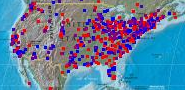
\includegraphics[scale=1.25]{gd_detail}\medskip
		
		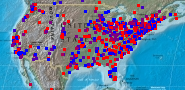
\includegraphics[scale=1.25]{html_detail}
	\end{center}
	\caption{Image quality of JPEG image generation (top) vs.\ HTML
	overlay (bottom).}
	\label{fig-image-quality}
\end{figure}


\subsection{Google Maps}
\label{sec-google}

This technique uses the client-side Google Maps API
\cite{Goog-M-2006-maps} to both generate the base map and plot points on
it; an example of the output is shown in Figure~\ref{fig-google}. The
output and interaction is significantly different in nature from that
provided by the other two techniques. Google Maps requires JavaScript
support at the client and the Google Maps software must be installed on
the client. However, since the latter happens automatically when the
corresponding web page is loaded, this technique meets our requirements.
Google Maps inherently uses a distributed architecture, as shown in
Figure~\ref{fig-google-architecture}. Data are generated at the server,
while all map display and manipulation occurs at the client.


\begin{figure}
	\begin{center}
		\includegraphics[width=0.95\textwidth,keepaspectratio]{google_map}
	\end{center}
	\caption{Sample output from the Google Maps technique.}
	\label{fig-google}
\end{figure}


\begin{figure}
	\caption{Distributed architecture of the Google Maps technique.}
	\label{fig-google-architecture}
\end{figure}


The primary advantage of this technique is the powerful functionality it
provides for generating and interacting with the map. Users may pan the
map in any direction and zoom in and out to many different levels. A
satellite imagery view is also available. In addition, further
information about each point plotted (such as the name of the city, for
example) can be displayed in a ``speech bubble'' next to the point, as
shown in Figure~\ref{fig-google}. The display is also visually appealing.

However, there are also some significant disadvantages compared to the
previous two techniques. As a distrbiuted applicatiopn, it is more
complex to implement and debug. It also relies on an active Internet
connection in order to run. The server must register an API key with
Google, which is checked every time that a page attempts to use the API.
Similarly, the client must connect to Google's servers in order to to
download the API's JavaScript source. Consequently, this technique
cannot be used on an isolated network. Finally, the Google Maps API does
not currently provide any method of toggling the visibility of markers
on the map, so it is not possible to implement the ``layers'' that are
possible with the HTML overlay technique (it is of course possible that
Google will implement this feature in a later version of the API).

Interestingly, the Google Earth application addresses several of these
issues, but falls outside the scope of this work, as it requires the
manual installation of extra software and runs outside the web browser
entirely. (Just for fun, however, we will do an informal comparison in
Section~\ref{sec-results} between Google Earth and the three techniques
discussed here.)


\section{Experimental design}
\label{sec-experiment}

After some preliminary experimentation and testing with live data from
the Otago School of Business repository, we proceeded with a more formal
series of experiments to test the scalability of the three techniques.
Each technique was tested using progressively larger sets of synthetic
data. The first data set comprised one point at the South Pole (latitude
\(-90^{\circ}\), longitude \(0^{\circ}\)). Each successive data set was twice
the size of its preceecssor, and comprised a regular grid of
latitude/longitude points at one degree intervals. A total of twenty-one
data sets were created in this way, with the number of points ranging
from one to 1,048,576 (\(=2^{20}\)).

Beacuse of the focus on scalability, we were primarily interested in
measuring page load times, memory usage, and the amount of data
generated (which impacts on both storage and network bandwidth). The
page load time can be further broken down into the time taken to
generate the map data, the time taken to transfer the map data to the
client across the network, and the time taken by the client to display
the map.

Unfortunately, the Google Maps technique requires an active Internet
connection, so we were unable to run the experiments on an isolated
network. This meant that traffic on the local network could be a
confounding factor. We therefore decided to eliminate network
performance from the equation by running both the server and the client
on the same machine\footnote{A Power Macintosh G5 1.8\,MHz with 1\,GiB
RAM, running Mac OS X 10.4.7, Apache 2.0.55, PHP 4.4 and Perl 5.8.6.}.
This in turn enabled us to measure the time taken for data generation
and page display independently of each other, thus simplifying the
process of data collection and also reducing the impact that the client
and server processes would have on each other.

It could be argued that network performance would still have a
confounding effect on the Google Maps technique, but this would only be
likely for the intial download of the API (which comprises about
155\,KiB of JavaScript source), as the API will be locally cached
thereafter. The API key verification occurs every time the map is
loaded, but the amount of data involved is very small, so it seems
unlikely that this would be significantly affected by network
performance.

For each data set, we recorded the size of the data set, the time taken
to generate it, the time taken to display the resultant map in the
browser, and the amount of memory used during the test by both the
browser and the web server. The data set generation time and memory
usage were measured using the \texttt{time} and \texttt{top} utilities
respectively. The map display time was measured using the ``page load
test'' debugging feature of Apple's Safari web browser, which can
repetitively load a set of pages while recording various statistics, in
particular the time taken to load the page. Tests were run up to twenty
times each, where feasible, in order to reduce the impact of random
variations.

%%!! confused!

The image generation technique was implemented as a server-side
architecture. A dispatcher page written in PHP called a Perl script,
which generated a JPEG-compressed map image and returned this to the
browser.

The HTML overlay technique was implemented in two ways:
\begin{itemize}

	\item as a server-side architecture that worked in much the same way
	as the image generation technique, except that the Perl script
	returned an HTML file containing the \verb|<DIV>| elements for the
	overlay, and an \verb|<IMG>| element to load the base map image; and
	
	\item as a distributed architecture, where client-side JavaScript
	code made an asynchronous call to the server-side Perl script, which
	returned

and Google Maps techniques were implemented as a server-side
and a distributed architecture respectively. The HTML overlay technique
was implemented twice; once as a server-side architecture and once as a
distributed architecture.


\section{Results}
\label{sec-results}


\subsection{Data size}


\subsection{Display time}


\subsection{Memory usage}


\section{Conclusion}



% The
% software extracts IP addresses from the web server logs, geolocates them
% using the free MaxMind GeoLite Country database\footnote{See
% \url{http://www.maxmind.com/app/ip-location}.}, then stores the
% resulting country information in a separate database.

% The Tasmania software, however, uses countries as its base unit of
% aggregation. We were interested in looking at the distribution on a finer
% level, down to individual cities if possible


\bibliography{Map_Visualisation}

\begin{received}
...
\end{received}
\end{document}


